%
% main.tex -- Paper zum Thema Eis
%
% (c) 2018, Silvio Marti, Hochschule Rapperswil
%
\chapter{Eis\label{chapter:eis}}
\lhead{Eis}
\begin{refsection}
\chapterauthor{Silvio Marti}

\section{Einleitung}
\rhead{Einleitung}
Diese Arbeit befasst sich damit, wie die Anwesenheit von Eis an den Polen modelliert werden kann. Immer wieder hört man, dass das Polareis rasant schmilzt und der Eisschwund ein bedrohliches Ausmass angenommen hat. Als Grund wird jeweils die globale Erwärmung genannt. Das scheint plausibel, denn wie man schon im Modell von Budyko <<Verweis Budyko>> sehen kann, gilt für eine höhere Gleichgewichtstemperatur ein tieferer Albedo, was bedeutet, dass es weniger reflektierendes Eis geben muss. Es sei aber betont, dass die Kurve Albedo(T) <<Verweis auf Grafik Albedo(T)>> sich nur auf die beiden Punkte $Snowball\text{ }earth$ ($T$ = 250K, Albedo = 0.7) und $kein\text{ }Eis$ ($T$ = 280K, Albedo = 0.3) stützt und dazwischen mit einer willkürlich gewählten $tanh$ Funktion modelliert wurde. 
\subsection{Eisschmelze am Nordpol}
\rhead{Eisschmelze am Nordpol}
Um eine Idee über das Ausmass der Eisschmelze in den letzten 25 Jahren zu bekommen, dient die folgende Grafik:%
	\footnote{\url{https://svs.gsfc.nasa.gov/4510}}
\begin{figure}[H]
	\centering
	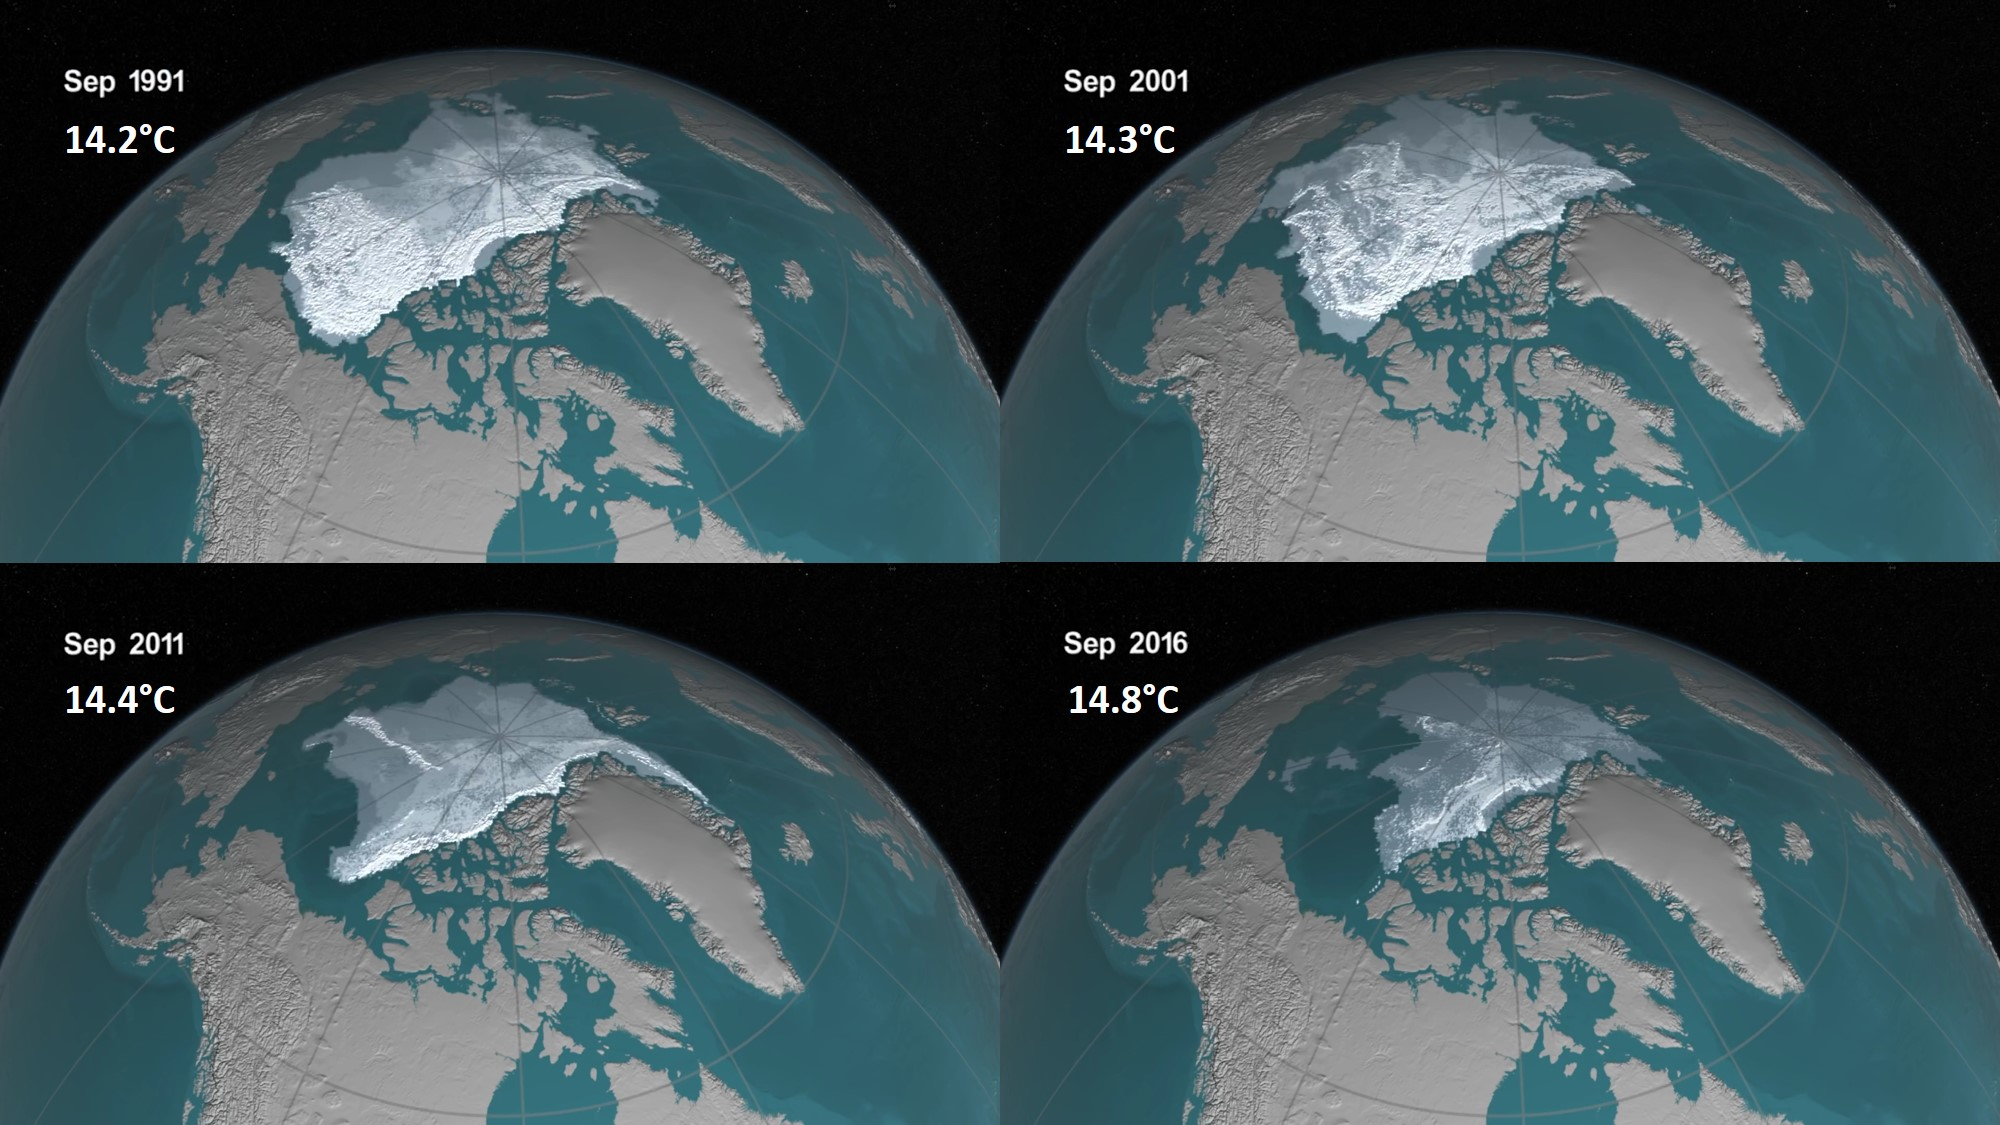
\includegraphics[width=14cm]{eis/NASA_ohne_Breitengraden.jpg}
	\caption{Ausschnitt aus einer Animation der NASA. Dargestellt ist das Polareis (nur das Meereis, ganz Grönland ist z.B. auch vereist) jeweils im September des angegebenen Jahres. Je weisser das Eis, desto älter ist es (ganz weiss entspricht vier Jahre und älter).	Dazu ist auch die globale Jahresdurchschnittstemperatur eingetragen.}
	\label{skript:eis:fig:NASAohne}
\end{figure}
Die nächste Grafik zeigt die Veränderung der globalen Durchschnittstemperatur über einen ähnlichen Zeitraum. Obwohl es wenig Sinn macht, diese Werte absolut anzugeben, wollen wir das hier tun; wir sehen in Kapitel \ref{skript:Eis:Resultate} die Verwendung. Die Referenz, um aus den differenziellen Werten \footnote{\url{https://climate.nasa.gov/vital-signs/global-temperature/}} absolute zu bekommen, ist das Jahr 2017, in welchem die Temperatur 14.7°C
\footnote{\url{https://www.ecmwf.int/en/about/media-centre/news/2018/2017-extends-exceptionally-warm-period-first-complete-datasets-show}} betragen haben soll.
\begin{figure}[H]
	\centering
	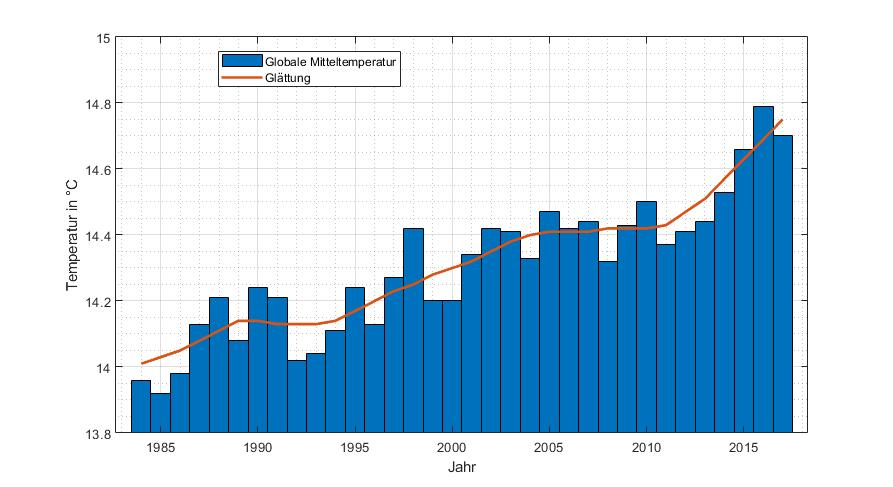
\includegraphics[width=14cm]{eis/globale_Mitteltemperaturen.jpg}
	\caption{Globale Durchschnittstemperatur 1984 bis 2017}
\end{figure}
\subsection{Problem an der Eisschmelze}
\rhead{Problem an der Eisschmelze}
Warum sind den Polkappen eine so grosse Bedeutung für das Klima zuzuschreiben? Probleme für das Klima einer grossen Eisschmelze aufgrund einer Temperaturerhöhung sind folgende: 
\begin{itemize}
	\item Wenn das Eis schmilzt, kommt irgendwann der darunterliegende Grund zum Vorschein. Das führt dazu, dass der Albedo an diesen Stellen sofort um mehr als die Hälfte sinkt, was bedeutet, dass global betrachtet die aufgenommene Strahlungsleistung zunimmt und die Erwärmung weiter vorantreibt.
	\item Taut Permafrost auf, gelangen grosse Mengen Methan, welche zuvor eingeschlossen waren, in die Atmosphäre, was ebenfalls zu einer zusätzlichen Erwärmung führt.
\end{itemize}
Veränderungen der Eismenge verstärken sich also von selbst.
Die Eisschmelze ist somit ein Prozess mit einer Mitkopplung mit globalen Auswirkungen.
Entscheidend für die genannten Prozesse ist nicht die Dicke des Eises, sondern die Fläche. Wie in Abbildung \ref{skript:eis:fig:NASAohne} zu erkennen ist, befindet sich das Eis ungefähr innerhalb eines Kreises um die Pole. Der Begriff $ice\text{ }line$ meint denjenigen Breitengrad, wo die Grenze der Vereisung ist.
\index{ice line}%
Alle darüber liegenden Breitengrade sind als vereist zu betrachten, die darunter nicht.
\section{Ziel}
\rhead{Ziel}
Offensichtlich existiert ein Zusammenhang zwischen der globalen Temperatur und der vorhandenen Eisfläche bzw. der ice line. Das Ziel ist, einen mathematischen Zusammenhang zu finden, um Aussagen über zukünftige Entwicklungen zu machen.
\section{Problem von Budyko}
\rhead{Problem von Budyko}
Budykos Modell konnte die Eisschmelze an den Polen nicht darstellen, bzw. aufgrund der nur geschätzten Albedo(T) tanh-Kurve keine präzise Aussage über die Eisfläche machen. Das Problem besteht darin, dass in diesem Modell folgende globale Annahmen getroffen wurden.
\begin{itemize}
	\item Gleichmässige Land und Wasserverteilung
	\item Gleichmässige Eisverteilung
	\item Gleichmässige Einstrahlung
	\item Gleichmässige Temperaturverteilung
\end{itemize}
\section{Modellverbesserung: Zonale Energiebilanz}
\rhead{Modellverbesserung: Zonale Energiebilandz}
Offensichtlich entsprechen diese Annahmen nicht der Realität. Besonders die Eisverteilung beschränkt sich wie definiert nur auf Gebiete oberhalb der ice line.
Wir möchten nun Budykos Modell in ein realistischeres überführen, in dem wir die Erde in Zonen (Breitengrade) aufteilen und die Überlegungen zonenabhängig durchführen. Berücksichtigen wollen wir:
\begin{itemize}
\item Sonneneinstrahlung abhängig vom Breitengrad
\item Sonneneinstrahlung abhängig von der Neigung der Erdachse
\item Albedo abhängig vom Breitengrad (ice line)
\end{itemize}
\subsection{Einstrahlung abhängig vom Breitengrad}
Die Gegenden um den Äquator erhalten mehr Energie als die polaren Regionen. Um diesem Fakt Rechnung zu tragen, führen wir die Breitengradabhängige Energieverteilungsfunktion $s(\theta)$ ein, wobei $\theta$ den Breitengrad bezeichnet.
\begin{equation}\label{Energieverteilung Breitengrad}
s(\theta)
=
\frac{2}{\pi^2}\int_{0}^{2\pi}cos(\theta)d\phi,\quad
\theta\in(-\tfrac{1}{2}\pi,\tfrac{1}{2}\pi)
\end{equation}
Der Faktor $\frac{2}{\pi^2}$ wird für die Normalisierungsbedingung in Kapitel "Verweis" verwendet. Wird nur der Breitengrad berücksichtigt, ergibt sich folgendes Bild.
\begin{figure}[H]
 	\centering
 	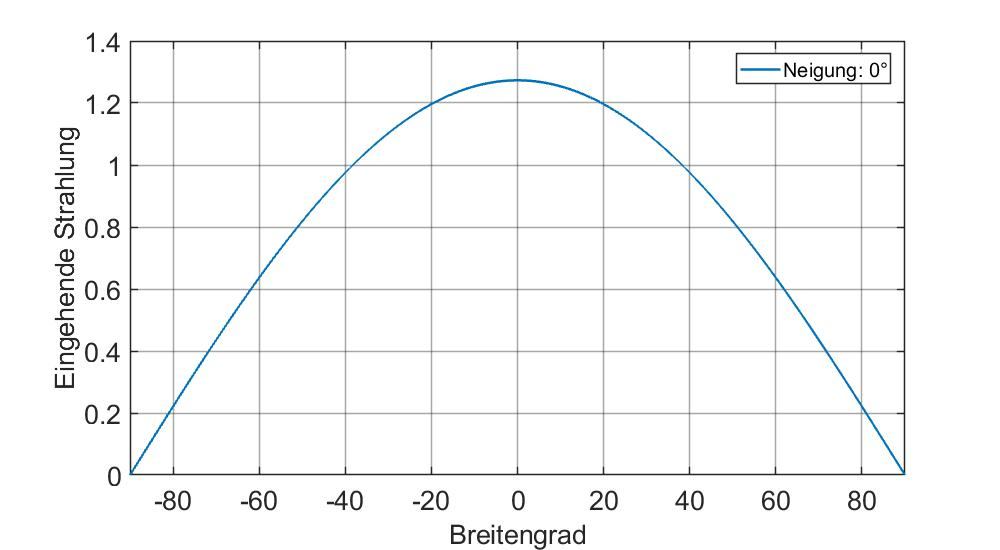
\includegraphics[width=10cm]{eis/Einstrahlung_abh_vom_Breitengrad.jpg}
 	\caption{Energieverteilung abhängig vom Breitengrad}
\end{figure}
\subsection{Einstrahlung abhängig vom Neigungswinkel}
Weil die Erdachse einen Neigungswinkel hat, geht die Sonne im Sommer im hohen Norden nicht unter, was bedeutet, dass auch die Pole Einstrahlung erhalten. Obige Grafik kann somit nicht stimmen, die Neigung $\beta$ muss berücksichtigt werden. Um dem Rechnung zu tragen, führen wir den Index $\beta$ ein und schreiben ab jetzt $s_{\beta}(\theta)$. Die Energieverteilungsfunktion ist jetzt gegeben durch ein elliptisches Integral.
\begin{equation}\label{Energieverteilung Neigung}
s_{\beta}(\theta)
=
\frac{2}{\pi^2}\int_{0}^{2\pi}\sqrt{1-(cos\theta sin\beta cos\phi-sin\theta cos\beta)^2}d\phi
\end{equation}
Es kann gezeigt werden, dass die Formel \ref{Energieverteilung Breitengrad} der Spezialfall für eine Neigung von $0^{\circ}$ ist. Zurzeit beträgt die Neigung $\beta=23.4^{\circ}$, damit verändert sich die Energieverteilung folgendermassen.
\begin{figure}[H]
	\centering
	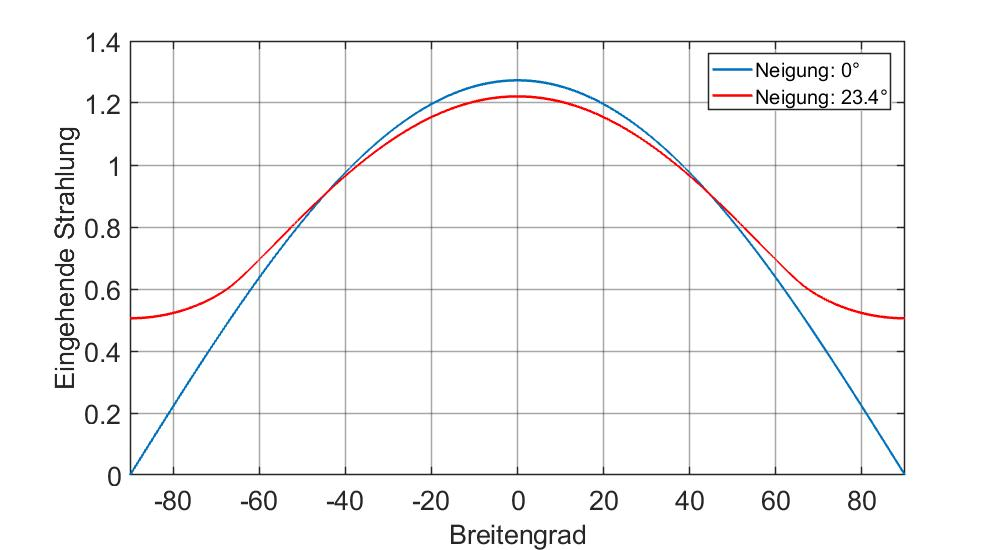
\includegraphics[width=10cm]{eis/Einstrahlung_abh_mit_und_ohne_Neigung.jpg}
	\caption{Energieverteilung abhängig vom Breitengrad und dem Neigungswinkel}
\end{figure}
Wichtig zu sehen ist hier, dass die Energie an den Polen eben nicht Null ist, der Einfluss der Neigung ist somit beträchtlich. Die saisonalen Schwankungen der ice line betragen über ein Dutzend Breitengrade. Aufgrund der Überlegungen über die Neigung wird jetzt auch klar, für welche Jahreszeit wir die ice line berechnen wollen. Im Winter, wenn keine Einstrahlung am Nordpol statt findet, wird auch keine Energie vom Eis reflektiert, dessen Ausbreitung verliert also im Winter an Bedeutung. Relevant für unser Modell ist also nur das Eis im Sommer. Weil es zu Beginn jeweils noch viel Eis vom Winter übrig hat, legen wir uns auf den Monat September fest, wo die Ausbreitung ihr Minimum erreicht. Sämtliche Resultate werden sich also auf den Spätsommer beziehen und geben die minimale jahreszeitenabhängige Vereisung an.
\subsection{Normalisierungsbedingung}
Bei den verwendeten Formeln muss sichergestellt werden, dass die eingestrahlte Leistung immer dieselbe ist. Sie darf nur verteilt, aber nicht verändert werden. Mir folgender Formel wird das überprüft:
\begin{equation}\label{Normalisierungsbedingung}
	\frac{1}{2}\int_{-\pi/2}^{\pi/2}s_{\beta}(\theta)cos\theta d\theta
	=
	1
\end{equation}
\subsection{Approximation}
Für die Breitengradabhängige Einstrahlung erweist es sich als mühsam, die Formel \ref{Energieverteilung Neigung} zu benutzen, weil für jeden Breitengrad das Integral aufgelöst werden muss. Die Funktion soll deshalb für eine fixe Neigung von $\beta=23.4^{\circ}$ approximiert werden. Selbstverständlich muss auch die Approximation die Normalisierungsbedingung \ref{Normalisierungsbedingung} erfüllen. Wir finden:
\begin{equation}\label{Energieverteilung Approximation}
	\tilde{s}(\theta)
	=
	0.523+0.716cos^{2}\theta
\end{equation}
Wie auf der nächsten Grafik zu sehen ist, deckt sich die Approximation gut mit der Originalfunktion.
\begin{figure}[H]
	\centering
	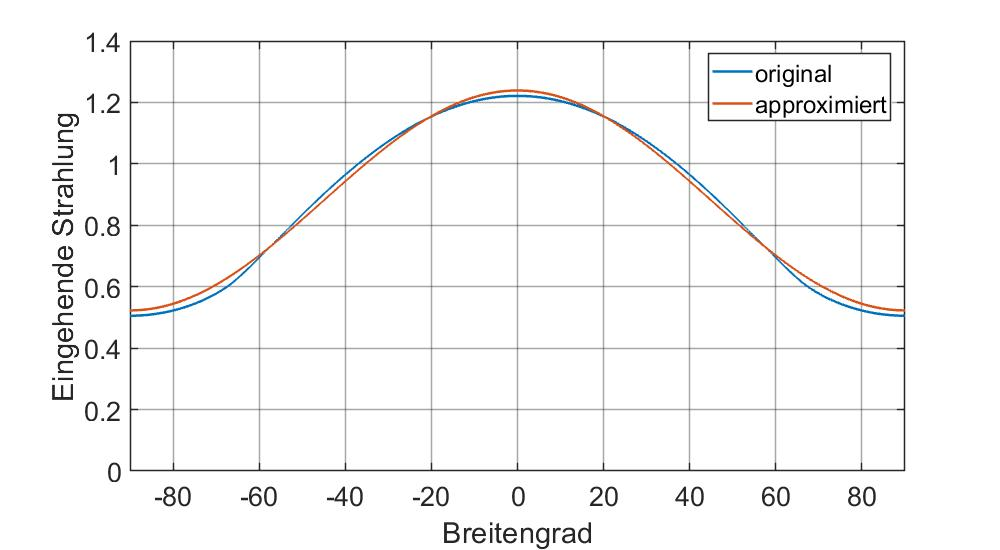
\includegraphics[width=10cm]{eis/Einstrahlung_approximiert_Vergleich.jpg}
	\caption{Vergleich der Energieverteilungsfunktion gemäss \ref{Energieverteilung Neigung} mit der Approximation \ref{Energieverteilung Approximation}}
\end{figure}
\subsection{Absorbtionsverteilung}
In den vereisten Breitengraden wird mehr Sonnenlicht reflektiert, der Albedo ist deshalb dort grösser als bei einer nicht vereisten Oberfläche. Gemäss der Definition in Kapitel \ref{Problem an der Eisschmelze} ergibt sich folgende Funktion für den Albedo $a$:
\begin{equation}\label{Albedoverteilung}
a(\theta,\theta_{iceline})
=
\begin{cases}
	0.7&-\tfrac{\pi}{2}\leq\theta\leq-\theta_{iceline}\\
	0.285&-\theta_{iceline}\leq\theta\leq\theta_{iceline} \\
	0.7&\theta_{iceline}\leq\theta\leq\tfrac{\pi}{2}
\end{cases}
\end{equation}
\section{Energiegleichung}
\rhead{Energiegleichung}
Nun haben wir alle Komponente zusammen, um sie wieder in Budykos Modell einzufügen. Unter der Berücksichtigung der Zonen ergibt sich folgende Gleichung für die eingehende Strahlung pro Breitengrad
\begin{equation}\label{Ein pro Breitengrad}
Ein(\theta,\theta_{iceline})
=
(1-a(\theta,\theta_{iceline}))\cdot\tilde{s}_{b}(\theta)\cdot Q,
\end{equation}
wobei $Q=\tfrac{1}{4}S_{0}$. Damit die gesamte einfallende Energie betrachtet werden kann, muss die Gleichung \ref{Ein pro Breitengrad} über alle Breitengrade integriert werden. Dafür wird die Normalisierungsbedingung \ref{Normalisierungsbedingung} verwendet. Wird alles eingesetzt, resultiert eine Gleichung, bei der $Ein$ nur noch abhängig von der ice line ist, was das Ziel war.
\begin{equation}\label{Ein abh ice line}
Ein(\theta_{iceline})
=
\frac{Q}{2}\int_{-\pi/2}^{\pi/2}(1-a(\theta,\theta_{iceline}))\cdot(0.523+0.716cos^2\theta)\cdot cos\theta d\theta
\end{equation}
Um die Gleichgewichtslösungen zu erhalten, setzen wir $Ein$ mit $Eout$ gleich wie in <<Verweis Skript>> und bekommen
\begin{equation}\label{Gleichgewichtsgleichung}
	Ein(\theta_{iceline})
	=
	\epsilon\sigma T^4,
\end{equation}
wobei $T$ in $^{\circ}K$ angegeben ist.
\section{Resultate} \label{Resultate}
\rhead{Resultate}
Durch Umformen und Auflösen der Gleichung \ref{Gleichgewichtsgleichung} können nun folgende Zusammenhänge gezeigt werden:
\subsection{Albedo abhängig von der ice line}
\rhead{Albedo abhängig von der ice line}
\begin{figure}[H]
	\centering
	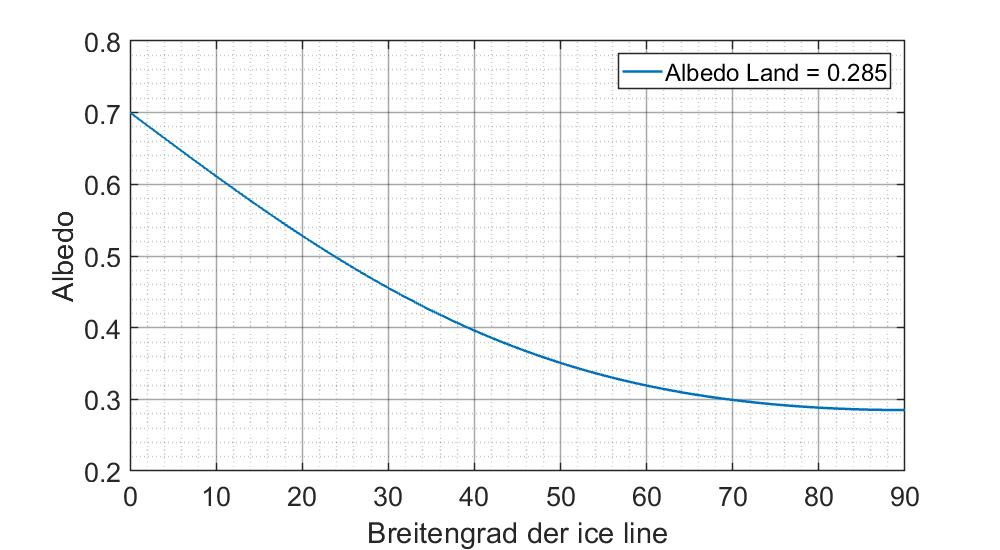
\includegraphics[width=14cm]{eis/Albedo_abh_von_der_ice_line.jpg}
	\caption{Globaler Albedo abhängig von der ice line. Ist die Erde zugefroren nimmt der globale Albedo den Wert des Eises an, existiert kein Eis, resultiert der Wert des Landes. Reduziert sich die Eismenge, fällt der Albedo monoton.}
\end{figure}
Wie schon im Modell von Budyko angenommen, ist hier klar ersichtlich, dass die Anwesenheit von Eis in den Polregionen nur wenig Einfluss auf den globalen Albedo hat. 
\subsection{Ice line abhängig von der Temperatur}
\rhead{ice line abhängig von der Temperatur}
\begin{figure}[H]
	\centering
	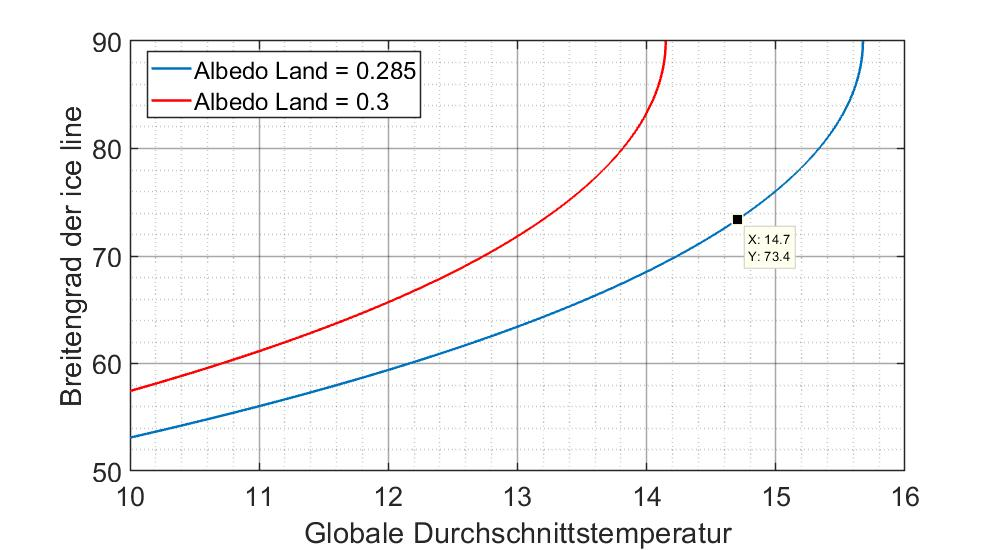
\includegraphics[width=14cm]{eis/iceline_abh_von_der_Temperatur_mit_Verleich_albedo_0,3.jpg}
	\caption{Abhängigkeit der ice line von der Temperatur für zwei verschiedene Werte vom Land Albedo. Der Messpunkt ist bei der Jahrestemperatur von 2017 eingetragen.}
\end{figure}
Diese Grafik zeigt sehr schön, wie sich die ice line bei einer globalen Erwärmung verhält. Gegen Ende reagiert sie sehr empfindlich auf eine Temperaturänderung, bis das Eis fast schlagartig verschwindet. Hier erklärt sich auch, warum für den Land Albedo der Wert 0.285 und nicht wie bei Budyko 0.3 verwendet wurde: Das Modell würde uns seit 20 Jahren kein Eis mehr anvertrauen, entsprechend musste der Wert so angepasst werden, dass es realistischer wird. Erwärmt sich die Erde weiter wie bis anhin, könnte das Polareis noch in diesem Jahrhundert vollständig verschwinden.
\subsection{Eisfläche abhängig von der Temperatur}
\rhead{Eisfläche abhängig von der Temperatur}
Ist die ice line bekannt, kann daraus mit folgender Formel die Eisfläche am Nord- und Südpol berechnet werden
\begin{equation} \label{Eisfläche}
	A_{Eis}=2\cdot 2\pi R^2(1-sin\theta),
\end{equation}
wobei $R$ dem Polradius von 6356km entspricht.
\begin{figure}[H]
	\centering
	\includegraphics[width=14cm]{eis/Eisfläche_abh_von_der_Temperatur.jpg}
	\caption{Zusammenhang der globalen Eisfläche und der Durchschnittstemperatur. Die Datenpunkte sind für die Temperatur vom Jahr 2017 und für eine zusätzliche Erwärmung von $0.5^{\circ}$.}
\end{figure}
Etwas unerwartet zeigt sich, dass dieser Zusammenhang beinahe linear ist. Bei einer Erwärmung ausgehend vom Jahr 2017 um weitere $0.5^{\circ}$C schmelzen 10 Mio. km$^2$ Eis, was rund $\tfrac{1}{50}$ der Erdoberfläche entspricht! Diese Zahlen stimmen aber so nicht wirklich, weil innerhalb der ice line doch nicht alles vereist ist. Sie zeigen aber die drastischen Auswirkung einer geringen Temperaturerhöhung.
\subsection{Vergleich mit der Realität}
\rhead{Vergleich mit der Realität}
Wie gut stimmt das Modell mit der Realität überein? Wir wollen dafür wieder die Bilder der NASA anschauen und die Daten des Modells einfügen.
\begin{figure}[H]
	\centering
	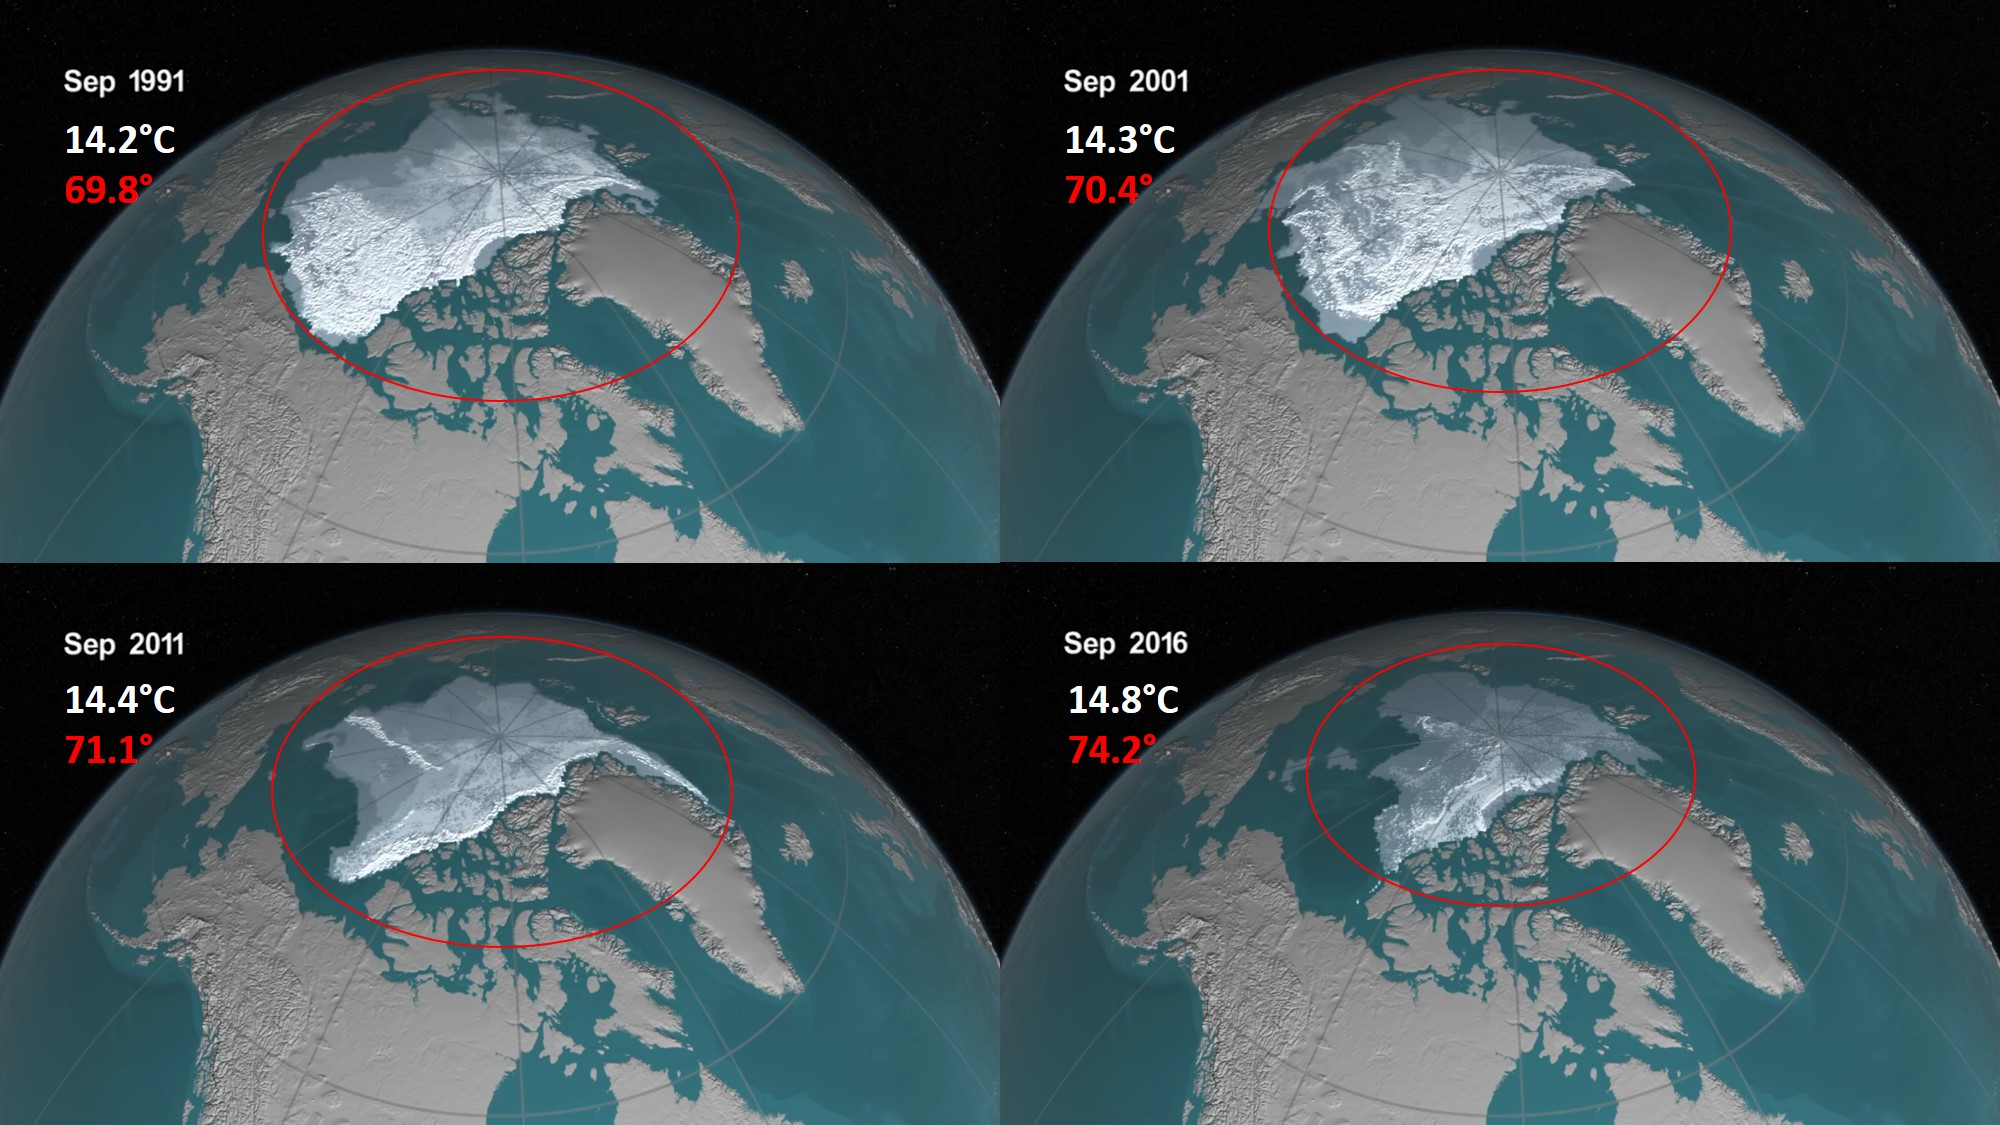
\includegraphics[width=14cm]{eis/NASA_mit_Breitengraden.jpg}
	\caption{Siehe Abb. \ref{skript:eis:fig:NASAohne}.
	Vergleich der Eisflächen mit der für die angegebene Durchschnittstemperatur berechneten ice line.}
\end{figure}
Besonders in der Region Alaska und Kanada ist die Übereinstimmung gut, an anderen Orten, wie über Skandinavien, deutlich schlechter, dort hat der Golfstrom einen grossen Einfluss. Zu beachten ist, dass ganz Grönland auch vereist ist. Das Modell kann also die Eisschmelze der letzten Jahre beschreiben, es scheint somit auch für zukünftige Temperaturen brauchbare Prognosen zu liefern.
\section{Modellfehler}
\rhead{Modellfehler}
Obwohl das Modell plausible Resultate liefert, wollen wir hier über die Fehler und getroffenen Annahmen diskutieren. Folgende Punkte sind dabei besonders wichtig:
\begin{itemize}
	\item Kein Wärmefluss. Sämtlicher Energieaustausch zwischen den Breitengraden in Form von Wärmeleitung und besonders von Konvektion durch die Meeresströmungen wurde unterbunden. Dies wird die grösste Fehlerquelle im Modell sein.
	\item Symmetrie (ungleiche Land und somit Eisverteilung Nord/Süd). Um den Nordpol hat es bedeutend mehr Landfläche, als am Südpol. Deshalb darf im Norden mehr Eis erwartet werden, weil das Land schneller gefriert und sich Permafrost bildet, als sich auf dem Meer Eis. Ausserdem unterbrechen Landmassen die Meeresströmungen und erschaffen so eine polare Klimazone.
	\item Die abgestrahlte Leistung ist auch Temperatur und somit Breitengradabhängig. Indem wir Zonen mit und ohne Eis haben, lassen wir implizit eine Temperaturverteilung zu. Weil die abgestrahlte Leistung proportional zu $T^4$ ist, wird an den Polen bestimmt nicht gleich viel Energie abgestrahlt, wie am Äquator.
	\item Keine Wärmekapazität. Dies führt dazu, dass keine Jahreszeiten abgebildet werden können; die ice line schwankt über das Jahr um über ein Dutzend Breitengrade. Das Eis mittelt Temperaturschwankungen auch über mehrere Jahre aus.
	\item Approximationen. Zu guter Letzt sei erwähnt, dass die Energieverteilung mit der Gleichung \ref{Energieverteilung Approximation} approximiert wurde. Der Einfluss auf das Ergebnis dürfte aber gering ausfallen.
\end{itemize}
\section{Schlussfolgerung}
\rhead{Schlussfolgerung}
Anhand der Betrachtungen können folgende Aussagen gemacht werden:
\begin{itemize}
	\item Es kann ein einfaches Modell berechnet werden, welches einen Zusammenhang zwischen der ice line und der globale Durchschnittstemperatur herstellt.
	\item Das Modell erweist sich im Vergleich zu den Aufnahmen der NASA als plausibel.
	\item Die ice line reagiert sehr empfindlich auf eine Temperaturänderung! Bei der Eisfläche sieht es weniger schlimm aus. 
\end{itemize}
Mit Sicherheit kann gesagt werden, dass das Eis an den Polen zukünftig noch mehr zurückgehen wird, wenn sich die Erde weiterhin erwärmt. Es ist denkbar, dass wir einmal einen im Sommer eisfreien Nordpol noch erleben könnten. Die gute Nachricht dabei: Das Modell macht keine Aussage darüber, dass der Prozess der Eisbildung nicht reversibel wäre. Sollte sich die Erde also wieder abkühlen, wird es wieder mehr Eis geben.
\printbibliography[heading=subbibliography]
\end{refsection}
